\section{Introducción}

\begin{frame}\frametitle{Filtros}
    \begin{figure}
        \centering
        \small
        \begin{tikzpicture}
          \node[bloque,minimum width=15mm] (T) {H($\cdot$)};
          \node (x) [left=of T] {};
          \node (y) [right=of T] {};
          \draw[arrow,->] (x.east) -- (T.west) node [midway,above] {$x(\cdot)$};
          \draw[arrow,->] (T.east) -- (y.west) node [midway,above] {$y(\cdot)$};
        \end{tikzpicture}
    \end{figure}
    \begin{itemize}
        \item \alert{¿Qué es un filtro?}\vspace{0.1cm}
        \begin{itemize}\footnotesize
            \item<2-> Dispositivo que modifica selectivamente las frecuencias de una señal.\vspace{0.1cm}
            \item<3-> Consideramos sistemas LTI estables.\vspace{0.1cm}
            \item<4-> Caracterización mediante:
            \begin{itemize}\scriptsize
                \item<4-> Respuesta en frecuencia: \color{blue}$H(j\omega)$ \color{black} o \color{blue}$H(\textrm{e}^{j\omega})$\color{black} (continuo/discreto).\vspace{0.05cm}
                \item<4-> Respuesta impulso: \color{blue}$h(t)$ \color{black} o \color{blue}$h[n]$\color{black} (continuo/discreto).
            \end{itemize}
        \end{itemize}
    \end{itemize}
\end{frame}

\subsection{Filtros Ideales}

\begin{frame}\frametitle{Filtros Ideales}
    \begin{columns}[T]
        \begin{column}{5cm}
            \visible<1->{
                \scriptsize
                \centering{Filtro paso bajo}
                \vspace{0.1cm}
                $H(j\omega)\!=\!\left \{  \!\!\!\begin{array}{l} 1, \: \textrm{para } |\omega|\!\!<\!\!\omega_c\\0, \:\textrm{c.c.}  \end{array}\right .$
                \vspace{-0.4cm}
                \begin{figure}
                    \centering
                    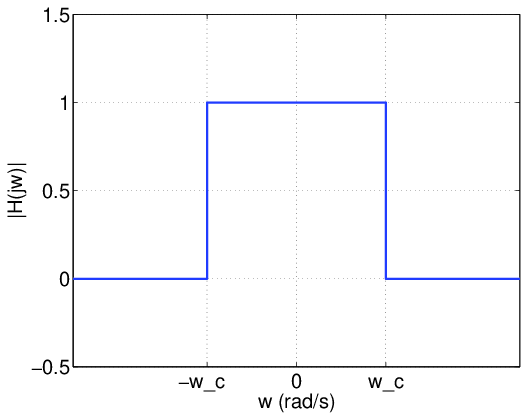
\includegraphics[width=3.2cm]{Figures/FiltroPBaja.png}
                \end{figure}
                \vspace{-0.2cm}
            }
            \visible<2->{
                \scriptsize
                \centering{Filtro paso alta}
                \vspace{0.1cm}
                $H(j\omega)\!=\!\left \{  \!\!\!\begin{array}{l} 0, \: \textrm{para } |\omega|\!\!<\!\!\omega_c\\1, \:\textrm{c.c.}  \end{array}\right .$
                \vspace{-0.4cm}
                \begin{figure}
                    \centering
                    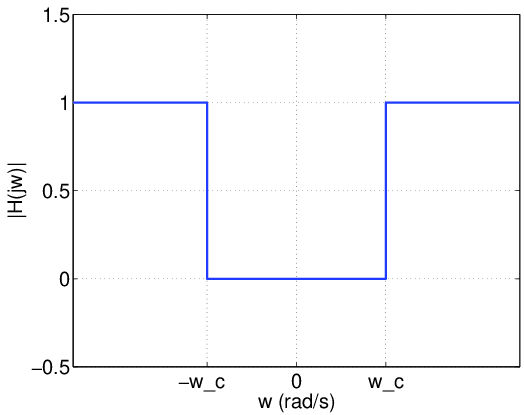
\includegraphics[width=3.2cm]{Figures/FiltroPAlta.png}
                \end{figure}
                \vspace{-0.2cm}
            }
        \end{column}
        \begin{column}{5 cm}
            \visible<3->{
                \scriptsize
                \centering{Filtro paso banda}
                \vspace{0.1cm}
                $H(j\omega)\!=\!\left \{  \!\!\!\begin{array}{l} 1, \:  \omega_{c_1}\!\!<\!\!\omega\!\!<\!\!\omega_{c_2}\\0, \:\textrm{c.c.}  \end{array}\right .$
                \vspace{-0.4cm}
                \begin{figure}
                    \centering
                    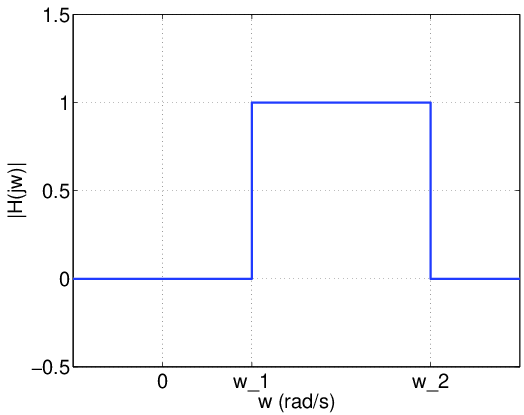
\includegraphics[width=3.2cm]{Figures/FiltroPBanda.png}
                \end{figure}
                \vspace{-0.2cm}               
            }
            \visible<4->{
                \centering{Filtro supresor banda}
                \vspace{0.1cm}
                $H(j\omega)\!=\!\left \{  \!\!\!\begin{array}{l} 0, \:  \omega_{c_1}\!\!<\!\!\omega\!\!<\!\!\omega_{c_2}\\1, \:\textrm{c.c.}  \end{array}\right .$
                \vspace{-0.4cm}
                \begin{figure}
                    \centering
                    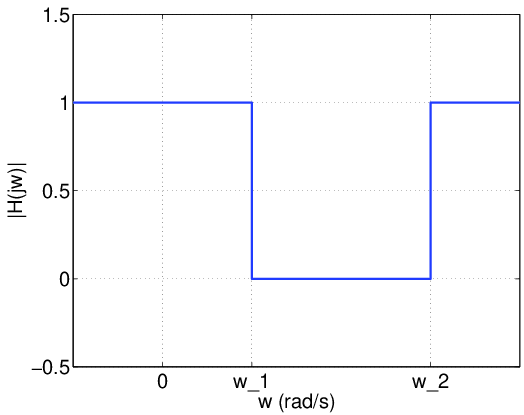
\includegraphics[width=3.2cm]{Figures/FiltroSBanda.png}
                \end{figure}
                \vspace{-0.2cm}
            }    
        \end{column}
    \end{columns}
\end{frame}